\chapter{Related work} \label{chap3}

\section{Bibliographical research methodology} \label{3biblio_research}

To define the state-of-the-art for ECG classification and Federated learning I performed a reduced Systematic Review. The latter is defined as \cite{systematic_review} a 'process of critically evaluating, summarizing, and seeking to reconcile the evidence.' In other words, it is a complete evaluation of literature that differs from a traditional review in that it is undertaken in a methodical (or systematic) manner, following a pre-specified process to avoid bias, with the goal of synthesizing the information gathered. 

Then the first step to perform the systematic review (SR or bibliographical research) was to decide the reference and citation databases to use. In the table \ref{table:dbs_sr} are written the academic search engines used to retrieve the related documents.

\begin{table}[H]
\begin{center}
% \resizebox{\textwidth}{!}{
\begin{tabular}{||p{0.2\linewidth} || p{0.55\linewidth} | p{0.15\linewidth}||}
 \hline
\textbf{Search Engine} & \textbf{Definition} & \textbf{Link} \\ [0.4ex] 
 \hline\hline
Google Scholar & A free web search engine that indexes the full text or metadata of scholarly literature from a variety of publishers and fields. & \href{https://scholar.google.com/}{Link to GS} \\
\hline
PubMed.gov & Contains almost 34 million citations from MEDLINE, life science journals, and online books for biomedical literature. & \href{https://pubmed.ncbi.nlm.nih.gov/}{Link to PM} \\
\hline
IEEEXplore & A research database that allows users to access journal articles, conference proceedings, technical standards, etc. in computer science, electrical engineering, and electronics. & \href{https://ieeexplore.ieee.org/Xplore/home.jsp}{Link to IE} \\
\hline
Scopus & Has a huge collection of Physical Sciences and Engineering papers, from foundational science to novel and unique research, and spanning many disciplines both theoretical and applied. & \href{https://www.sciencedirect.com/}{Link to SCs} \\
\hline
Web Of Science & It is the most reliable publisher-independent worldwide citation database in the world. & \href{https://clarivate.com/webofsciencegroup/solutions/web-of-science/}{Link to WoS} \\
\hline
Papers with code & Their goal is to provide a free and open library that includes Machine Learning articles, code, datasets, methodologies, and evaluation tables. & \href{https://paperswithcode.com/}{Link to PwC} \\
\hline\hline
\end{tabular}
% }
\end{center}
\caption{Databases (search engines) used to find documents}
\label{table:dbs_sr}
\end{table}

Each one of the search engines showed in the previous table work based on a "query" which will contain the information of the topic desired. Besides, to get better results, it is recommended to use multiple queries that may enrich the matter in research. Those queries are listed below, grouped by the specific topic to be found about:

\begin{enumerate}
    \item \textbf{Federated learning Generalities}: To retrieve the conceptual definition and approximations of Federated Learning I used the following queries:
    \begin{itemize}
        \item Federated learning arrhythmia
        \item Federated learning ECG
        \item Federated learning healthcare arrhythmia
        \item Federated learning healthcare iot
        \item Federated learning IoT ecg
        \item Federated learning healthcare low power mobile
        \item Federated learning PhysioNet
        \item Federated learning TensorFlow Lite
    \end{itemize}
    \item \textbf{Options for ECG classification}: To get the different methods used along the history in the ECG classification theme I employed the next queries:
    \begin{itemize}
        \item Machine Learning ECG arrhythmia
        \item Deep Learning ECG arrhythmia
        \item Machine Learning IoT ECG arrhythmia
        \item Deep Learning IoT ECG arrhythmia
    \end{itemize}
    \item \textbf{Non-IID Methods}: To evaluate the different methods to deal with Non Independent Nor Identical distributed (Non-IID) data, I search over the following queries:
    \begin{itemize}
        \item Federated learning non iid
        \item Federated learning independent identically distributed
    \end{itemize}
    \item \textbf{Imbalanced data}: To check the techniques used b other authors regarding the class (labels, response variable) imbalanced, I used the next queries:
    \begin{itemize}
        \item Imbalanced data ecg
        \item Imbalanced data federated learning
    \end{itemize}
    \item \textbf{Metrics}: To gather the most used metrics in both ECG and Federated Learning ECG classifications I employed the following queries:
    \begin{itemize}
        \item Federated learning metrics
        \item ECG classification metric
    \end{itemize}
    \item \textbf{Federated learning types}: To understand the possible architectures of Federated Learning I was based on the next queries:
    \begin{itemize}
        \item Federated learning architecture
        \item Types federated learning
    \end{itemize}
    \item \textbf{Arrhythmia types}: To know the different arrhythmia classifications, I employed the following query:
    \begin{itemize}
        \item Cardiac Arrhythmia types
    \end{itemize}
\end{enumerate}

To gather in a proper and technical way all the documents and paers found I employed the PRISMA Flow. As cited in \cite{prisma_flow}, the latter is a flow diagram to depict the flow of studies through the different phases of the systematic review. That tool widely used for reporting original systematic reviews. Thus, the PRISMA flow employed is depicted in Figure xx.

 \begin{figure}[H]
\centering
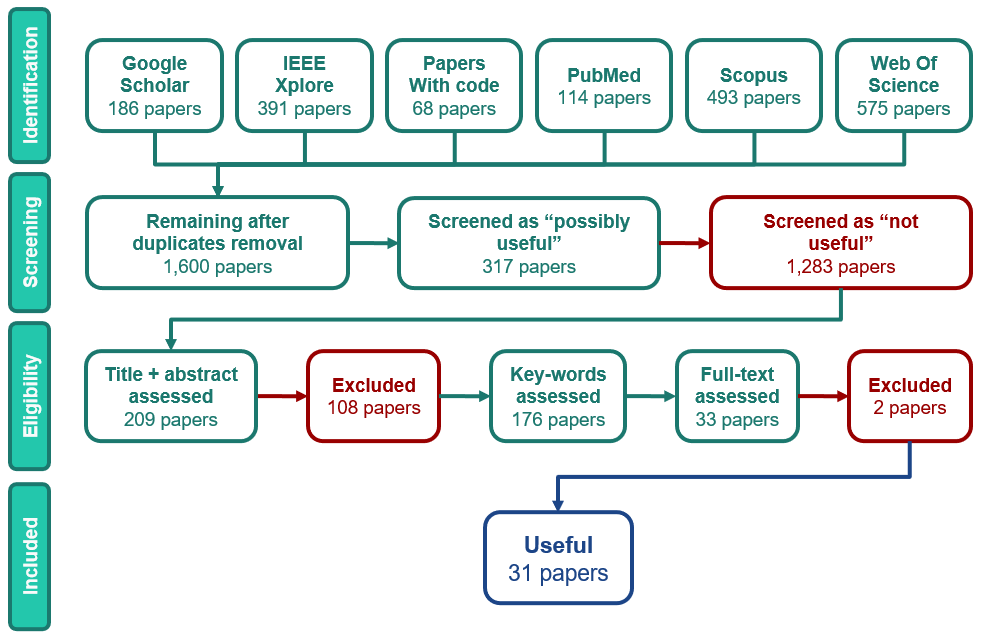
\includegraphics[scale=0.54]{img/prisma_flow.png}
\caption{Number of papers retrieved by year of publication and database}
\label{fig:prisma_flow}
\end{figure}

As shown in figure \ref{fig:prisma_flow}, along the phase of Identification, 1,827 articles where found using the queries mentioned previously. It is important to mention that for each one of those queries, I downloaded the results retrieved in BibTex and CSV formats, depending on the search engine used. With the files saved it was possible to retrieve some generalities from the documents. As an example, in figure \ref{fig:timeline_papers} it is depicted the number of papers found in each search database divided by publication year.

 \begin{figure}[H]
\centering
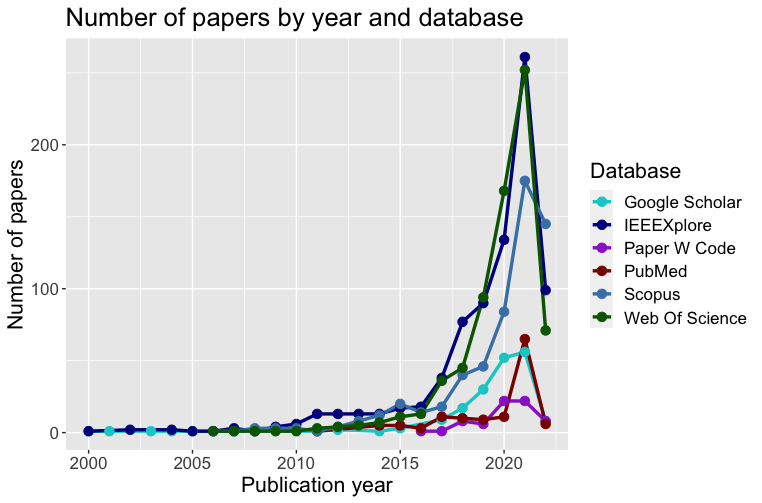
\includegraphics[scale=0.54]{img/timeline_papers.png}
\caption{PRISMA flow for gathering documents}
\label{fig:timeline_papers}
\end{figure}

From the previous graph we can see that most of the papers where published after 2017. That is because the concept of Federated Learning was introduced by Google in that year. Nevertheless, ECG classification is a topics that has been worked back in the 2000s. Moreover, the search engine that produced the highest number of resources was Web Of Science. 

Continuing with the analysis of figure \ref{fig:prisma_flow}, during the Screening phase I removed the duplicated documents keeping 1,600. After a fast screening (only title), I ended up with 317 possibly useful resources. During the eligibility phase, I screened the latter (title and abstract), ending up with 209 promising papers. Next, after assessing the keywords (given in the queries), I  reached 176 papers that were not read but were used to extract those keywords. On the other hand, I read 33 documents , from where 2 where not useful. That's the process how I found the 31 most useful papers after the research.

\section{ECG classification} \label{3state_art_ECG}

After reading the aforementioned documents, I gather some relevant highlights regarding the classification of ECG signals. Along the following paragraphs I summarize the most important findings at each topic.

\subsection{Techniques to handle imbalanced data}

In general, imbalanced data describes datasets in which the target class has an unequal distribution of observations. For example, when one class label has a large number of observations while the other has a small number.The authors who have dealt with this topic followed different paths to tackle this issue. Authors from \cite{imbalance_data1} introduced a \textit{Balanced Accuracy (BACC)} and the \textit{Matthew’s Correlation Coefficient (MCC)} to correct the fact that the classes don't share a similar distribution. In the article \cite{imbalance_data2} it was introduced the \textit{Generative Adversarial Network (GAN)} which deals with imbalanced data by generating and using additional fake data for detection purpose. In addition, \cite{imbalance_data3} used the \textit{Synthetic Minority Oversampling Technique (SMOTE)}, which is an oversampling technique. 

Other approaches also include the so-called \textit{Ratio Loss} (\cite{imbalance_data4}) where the global node estimates the composition data each round. When detecting an imbalanced composition continuously, the system acknowledges the class imbalance and load the Ratio Loss. One final possibility is the \textit{Recall of data} in which one randomly augment the lower class and in each training epoch change the selected individuals. Then, there are enough possibilities tried in the literature, each of of them with their pros and cons that can be verified further.



\subsection{Methods for ECG classification} \label{methods_ECG_class}

Along the literature I could find that a huge amount of diverse techniques have been applied when classifying ECG' arrhythmias. As an example \cite{ecg_methods1}, \cite{ecg_methods2}, and \cite{ecg_methods3} focused their efforts on Using Deep Neural Networks (Artificial Neural Networks and Multi-layer Perceptron) to get a model that predicts the abnormality given the ECG signal. In comparison, the author of \cite{ecg_methods4} combined in his paper the use of Naïve Bayes, Adaboost, Random Forest and Support Vector Machines to get the best classifier for his paper. Finally, \cite{ecg_methods5}, \cite{ecg_methods6} and \cite{ecg_methods7} employed in their research some Convolutional Neural Network approaches. Among them the highlighted Squeezenet, Attention mechanism and Resnet as the champion methods to deal with the ECG detection.

 \begin{figure}[H]
\centering
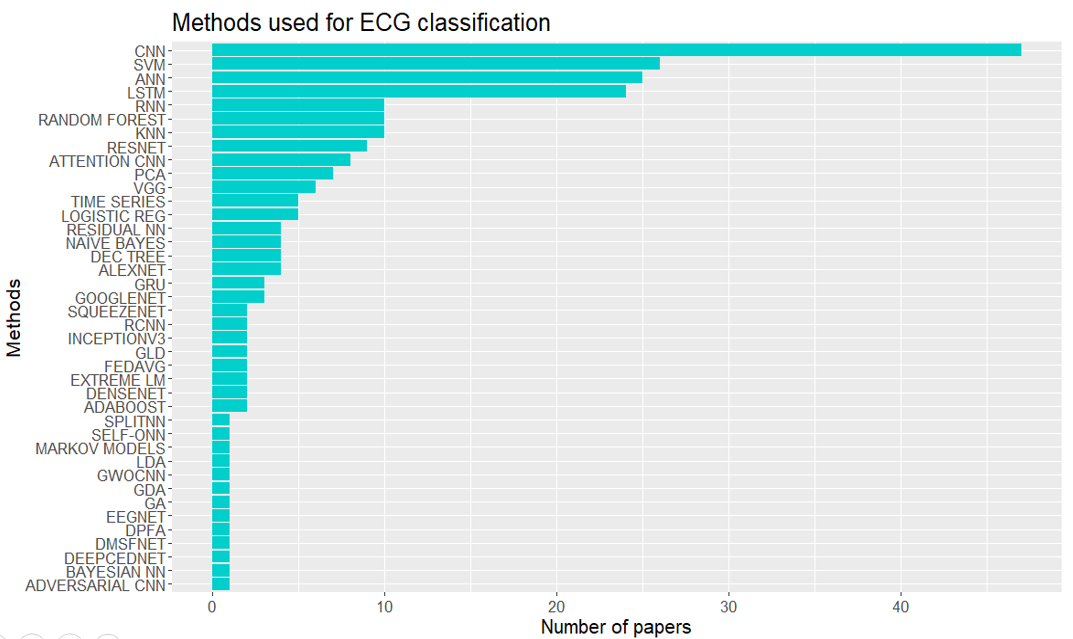
\includegraphics[scale=0.48]{img/classif_methods.PNG}
\caption{Most used classification methods for ECG}
\label{fig:classif_methods}
\end{figure}

As depicted in figure \ref{fig:classif_methods}, the most used technique is the Convolutional Neural Network (CNN). That one includes also some self-made Deep Neural Networks (DNN). On the second place we find Support Vector Machines (SVM) and Artificial Neural Networks (ANN). An very close to them most of the author also used Long-Short Term Memory (LSTM) algorithms. On the opposite, a few papers contributed with techniques like GWOCNN, DFPA, DEEPCETNET, etc, which are also CNN but that have specific alterations adapted to by the papers' authors.

\subsection{Metrics for ECG classification}\label{chap3metrics}

With respect to ECG arrhythmia classification, there are plenty of measurements employed in the literature. In figure \ref{fig:metrics_ECG} I show the most relevant metrics used in this aim, gathered from the available articles and papers shown in chapter \ref{3biblio_research}. 

 \begin{figure}[H]
\centering
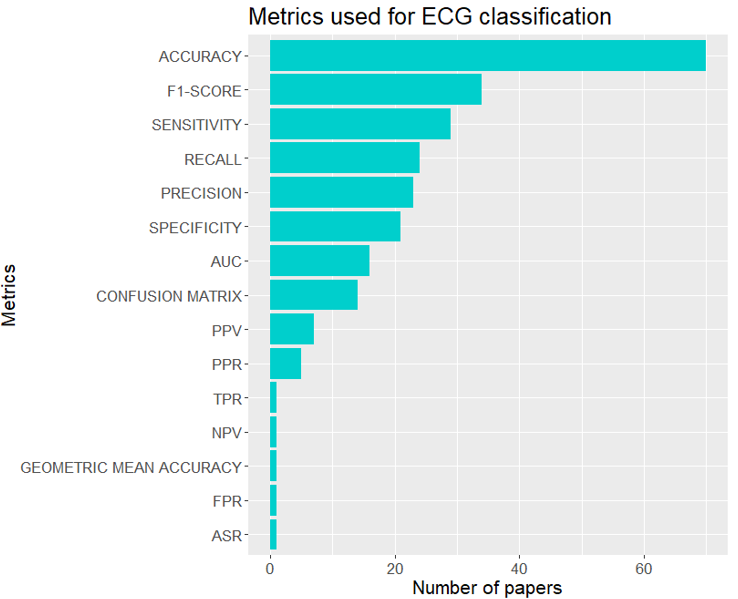
\includegraphics[scale=0.48]{img/metrics_ECG.PNG}
\caption{Most used metrics for ECG}
\label{fig:metrics_ECG}
\end{figure}

From the previous chart it is evident that the most used measure is the \textbf{Accuracy}. In the second place, the \textit{F1-Score} is often used. It is important to clarify that the latter is preferred when dealing with unbalanced data, since it take into account both \textit{Recall} and \textit{Precision} for its calculation. Some papers that consider the 4 mentioned measures at the same time can be found in \cite{metrics_ecg1}, 
\cite{metrics_ecg2} and \cite{metrics_ecg3}.


\section{Federated learning for ECG} \label{3state_art_FL}

Once provided materials in \cite{systematic_review} were assessed, I've compiled a list of key points about Federated Learning (FL) for ECG classification. I summarize the most important findings at each issue in the next paragraphs.


\subsection{Methods for ECG classification using Federated Learning}

In the ambit of Federated Learning (FL), most of the authors used Deep Neural Networks (DNN) and Convolutional Neural Networks (CNN). It has been noticed that traditional Machine Learning algorithms (like SVM, Random Forest, etc) are not usually employed for classify ECG signals in a FL context.

As an example, the authors of \cite{metrics_ecg1} used explainable artificial intelligence (XAI) and deep CNN to create a revolutionary end-to-end framework for ECG-based healthcare in a federated setting. With five-fold cross-validation, the trained classifier exceeded previous studies, attaining accuracy of up to 94.5 percent and 98.9 percent for arrhythmia diagnosis using noisy and clean data, respectively. In a federated scenario, they also presented a new communication cost reduction strategy that reduces communication costs while improving the privacy of users' data. The reported results can be found on figure \ref{fig:metrics_ecg1_results}.

\begin{figure}[H]
\centering
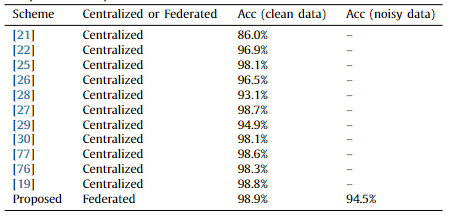
\includegraphics[scale=0.7]{img/metrics_ecg1_results.PNG}
\caption{Comparison with previous studies for ECG classification \cite{metrics_ecg1}}
\label{fig:metrics_ecg1_results}
\end{figure}

To save critical communication bandwidth, the paper \cite{fl2} adapted their suggested federated learning architecture for ECG analysis by asynchronously updating the shallow and deep model parameters of a proprietary CNN-based lightweight AI model. The results showed that the suggested asynchronous federated learning (Async-FL) approach can improve classification performance while simultaneously ensuring privacy, flexibility to new subjects, and reducing network bandwidth usage. Their proposed focus is in figure \ref{fig:fl2_focus}.

\begin{figure}[H]
\centering
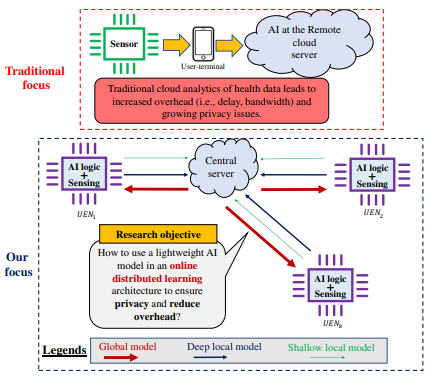
\includegraphics[scale=0.7]{img/fl2_focus.PNG}
\caption{The main focus was to do asynchronously
FL-based ECG method at the ultra-edge nodes (UENs) to classify ECGs preserving patient-data privacy\cite{fl2}}
\label{fig:fl2_focus}
\end{figure}

In order for Federated Learning to be performed on low-capacity devices in real-world settings, the authors of \cite{fl9} did an interesting job. For them, the training process must focus not only on achieving the highest level of accuracy, but also on lowering training time and resource consumption. In that study, they described a model training method that incorporates a dynamic epoch parameter. In Federated Learning, they offered the BePOCH (Best Epoch) algorithm to determine the optimal number of epochs every training round. In studies with medical datasets, they showed that using the BePOCH recommended number of epochs reduces training time and resource consumption while maintaining accuracy.

\begin{figure}[H]
\centering
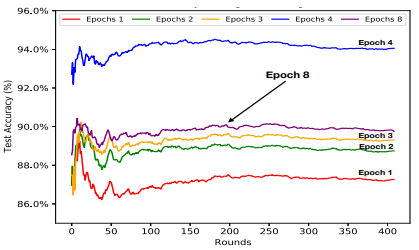
\includegraphics[scale=0.8]{img/fl9_epochs.PNG}
\caption{FL at various times throughout rounds. More epochs not always imply greater precision. Model with 8 epochs has a poorer accuracy than model with 4 epochs. \cite{fl9}}
\label{fig:fl9_epochs}
\end{figure}


\subsection{Methods to handle NON-IID data} \label{non_iid_handling}

Along the literature, the researches performed have been focused on tackling the Non Independent Nor Identical distributed (Non-IID) problem that make the models in FL under-perform. In the following part I present a summary of the most relevant techniques used to deal with the mentioned issue.

\textbf{Over/under-sampling}: This is one of the most common techniques used to balance the data. It consist of randomly creating (or removing) data to equate distributions. The simplest way to do it is called Random Oversampling (ROS). The latter is the process of randomly picking and replacing instances from the minority class in the training dataset. There are other techniques like SMOTE \cite{metrics_ecg1}. SMOTE is a data augmentation algorithm that creates synthetic data points depending on the original data points. The technique can be thought of as a more advanced variant of oversampling or as a specific data augmentation process. SMOTE has the advantage of not creating duplicate data points, but rather synthetic data points that are somewhat different from the original data points \cite{imbalance_data3}.

\begin{figure}[H]
\centering
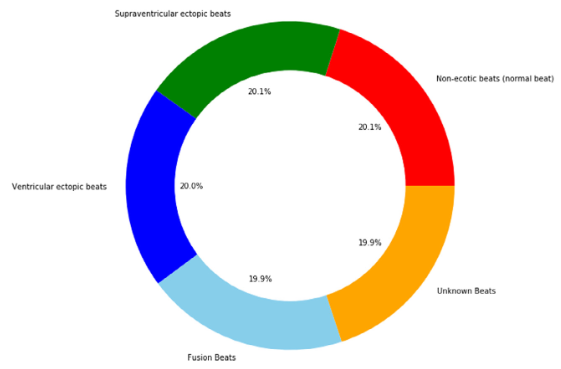
\includegraphics[scale=0.6]{img/metrics_ecg1_ROS.PNG}
\caption{The distribution of the up-sampled (re-balanced) dataset. \cite{metrics_ecg1}}
\label{fig:metrics_ecg1_ROS}
\end{figure}


\textbf{Data sharing strategy}: In the paper \cite{fl18} they showed that for neural networks trained with highly skewed non-IID data, where each client device trains just on a single class of data, the accuracy of federated learning drops by up to 55\%. They also showed that the weight divergence, which can be measured by the Earth mover's distance (EMD) between the distribution over classes on each device and the population distribution, can explain the loss in accuracy. As a solution, the proposal was to establish a limited sample of data that is globally shared across all edge devices to improve training on non-IID data. Their proposed data sharing is exposed in the following image:

\begin{figure}[H]
\centering
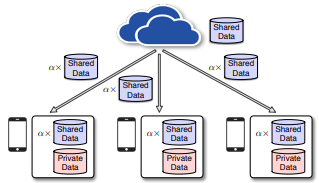
\includegraphics[scale=0.9]{img/fl18_datasharing.PNG}
\caption{ Illustration of the data-sharing strategy. \cite{fl18}}
\label{fig:fl18_datasharing}
\end{figure}

\textbf{Fedprox}: FedProx uses Federated Average Aggregation (FedAvg) to improve the local aim. It restricts the size of local updates directly. To limit the distance between the local model and the global model, it adds an additional L2 regularization term to the local objective function. This is a simple approach to keep the local updates under control so that the averaged model stays close to the global optima. To regulate the weight of the L2 regularization, a hyper-parameter is introduced \cite{fl19}.

\textbf{FedNova}: FedAvg is improved during the aggregation stage. Varying parties may undertake different numbers of local steps (i.e., the number of mini-batches in the local training) each round, according to the model. When parties have varying processing power under the same time restriction, or when parties have various local dataset sizes under the same number of local epochs and batch size, this can happen \cite{fl19}.

\textbf{SCAFFOLD}: uses the variance reduction technique to model non-IID as introducing variance among the parties. It introduces control variate for the server and parties, which are used to predict the server model's update direction and each client's update direction. The difference between these two update directions is then used to approximate the drift of local training. By include the drift in the local training, SCAFFOLD corrects the local updates \cite{fl19}.

\begin{figure}[H]
\centering
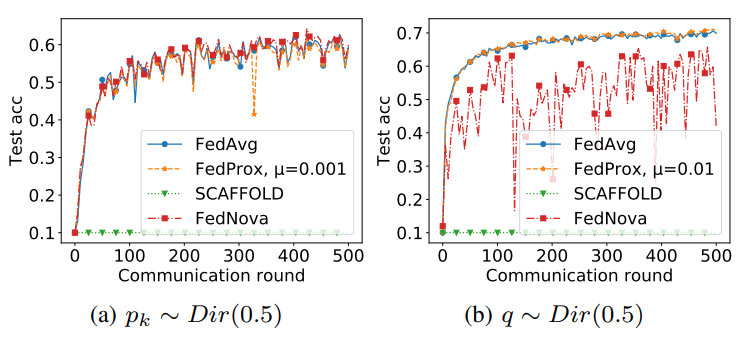
\includegraphics[scale=0.6]{img/fl19_fedprox.PNG}
\caption{Training curves of different approaches on CIFAR-10 with 100
parties and sample fraction 0.1. \cite{fl19}}
\label{fig:fl19_fedprox}
\end{figure}

\textbf{Classifier Calibration with Virtual Representations (CCVR)}:It uses virtual representations sampled from an estimated Gaussian mixture model to modify the classifier. On popular federated learning benchmarks including as CIFAR-10, CIFAR-100, and CINIC-10, experimental findings show that CCVR achieves state-of-the-art performance \cite{fl20}.

\begin{figure}[H]
\centering
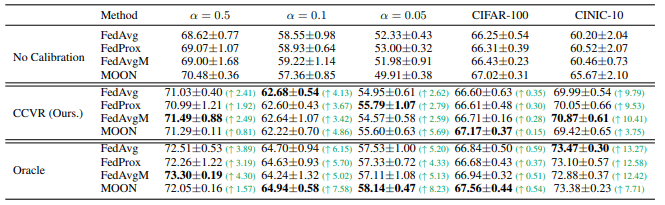
\includegraphics[scale=0.8]{img/fl20_CCVR.PNG}
\caption{Accuracy (\%) on CIFAR-10 with different degrees of heterogeneity ($\alpha$ $\in$ \{0.5, 0.1, 0.05\}), CIFAR-100 and CINIC-10. \cite{fl20}}
\label{fig:fl20_CCVR}
\end{figure}

\textbf{Federated Cloning-and-Deletion (FedCD)}: It is a learning system that involves iterative cloning of global models at predetermined milestones, adaptive updating of a high-scoring subset of global models, and deletion of poor-performing models to produce a specialized model for each archetype. Devices can self-select into groups with similar data by maintaining various global models and updating models that perform well on their local data. This allows for faster convergence as well as increased accuracy \cite{fl21}. 

\begin{figure}[H]
\centering
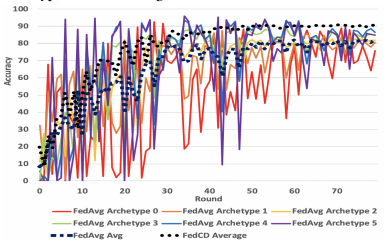
\includegraphics[scale=0.8]{img/fl21_fedCD.PNG}
\caption{Comparisons of test accuracy for the FedAvg and FedCD (dotted)
algorithms. \cite{fl21}}
\label{fig:fl21_fedCD}
\end{figure}

\textbf{Inverse Distance Aggregation (IDA)}: It is a new robust aggregation method that reduces inconsistency among updated local parameters caused by the NON-IID problem. The computation of the coefficients $\alpha_k$, which is based on the inverse distance of each client parameter to the average model of all clients, lies at the heart of that method. This enables the poisoned models, i.e. out-of-distribution models, to be rejected or weighed less heavily \cite{fl22}.

\begin{figure}[H]
\centering
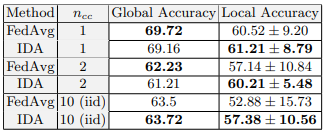
\includegraphics[scale=0.9]{img/fl22_IDA.PNG}
\caption{Investigation on unbalanced data distro. among the clients in FL, with 5 random classes per client, and random number of samples per client for HAM10k. \cite{fl22}}
\label{fig:fl22_IDA}
\end{figure}



\subsection{Metrics for Federated Learning}

Inside the FL framework the same metrics showed in \ref{chap3metrics} are often used. In the ECG case, metrics like Accuracy, F1-Score, Recall and Precision are usually employed to measure the overall capacity of the model to detect the diagnoses. In addition, with the introduction of FL, some new metrics are considered to determine the behaviour of the training stage while considering the local nodes. Those metrics are explained in the following sections.

The authors of \cite{fl23} provided a set of metrics for assessing individualized FL models in terms of performance and fairness. They computed the following metrics on the Quantum of Improvement (QoI) to quantify the per-user accuracy gains acquired in terms of personalization:

\begin{equation} \label{eq1}
\begin{split}
F_i = P_i - max(G_i, L_i)
\end{split}
\end{equation}

where P, G, and L relate to the personalized model's accuracy, FedAvg and local model of user I while $F_i$ refers to user i's QoI. In all equations, F will be referred as the QoI from now on.

The QoI can have unfavorable results. This suggests that the tailored method reduces the accuracy of a user's personalized model rather than increasing it as expected when compared to local or global models. In such instances, using evaluation measures directly may lead to erroneous results interpretation. As a result, there was a division of the QoI into two sets, each including the absolute QoI values: a set of positive QoI users (U+) and a set of negative QoI users (U-). The introduced measurements are then applied to both sets and interpreted accordingly.

\subsubsection{Performance Metrics}:
\textbf{Percentage of User-models Improved (PUI)}: It is the percentage of users that see an improvement in their local and global models. A personalized model should, in theory, increase the per-user accuracy of a large number of users.

\begin{equation} \label{eq2}
\begin{split}
PUI = \frac{COUNT(F_i)}{COUNT(U)} \times 100, \; i \in U \; (U: Users)
\end{split}
\end{equation}

\textbf{Median Percentage of Improvement (MPI)}: Calculated as Median(U+), where the \textit{Median()} function returns the input's median and U+ is the QoI of the group of users who improved their performance. A tailored model should have a high median of QoI values among users who improve.

\textbf{Average Percentage of Improvement (API)}: Measures the average percentage improvement among users who enhanced their performance (U+).

\begin{equation} \label{eq3}
\begin{split}
API = \frac{\sum_{i \in U^{+}}{F_i}}{len(U^{+})}
\end{split}
\end{equation}

In some cases, a customizing strategy does not improve users' local and global accuracy. In such instances, it is critical to disclose the personalized model's per-user accuracy decline. There was a definition of two metrics to evaluate the decreasing accuracy because this drop cannot be obtained from the improvement measurements (MPI and API).

\textbf{Median Percentage of Decrease (MPD)}: Calculated in the same way as MPI: Median(U-).

\textbf{Average Percentage of Decrease (APD)}: It is the average percentage reduction among users whose performance has reduced (U-).

\subsubsection{Fairness Metrics}: 

The aforementioned measures were extended to evaluate personalization strategies that produce better results in terms of fairness. Based on the relation reflected by the fairness metric, the QoI distribution among K users is more fair (uniform) under technique t than t' for two approaches t and t'.

\textbf{Average Variance (AV)}: The AV is a measurement of data spread. It is defined as follows:

\begin{equation} \label{eq4}
\begin{split}
AV = \frac{1}{K}\sum_{i =1}^{K}{(F_i(t) - \hat{F}(t))^2}
\end{split}
\end{equation}

A lower AV indicates that a tailored technique can provides more fairness (uniformity).

\textbf{Entropy}: A measure that considers the magnitude of the QoI values. It can be calculated as:

\begin{equation} \label{eq5}
\begin{split}
Entropy = -\sum_{i=1}^{K}{\frac{F_i(t)}{\sum_{i=1}^{K}{F_i(t)}} \log\left(\frac{F_i(t)}{\sum_{i=1}^{K}{F_i(t)}}\right)}
\end{split}
\end{equation}

A personalized technique with a bigger Entropy has a higher fairness potential.

\subsubsection{Physical Metrics:}

Some publications included metrics that deal with the physical part (with the actual devices). For example, \cite{fl24} provided the following measurements:

\textbf{CPU and Memory Consumption}: Figure \ref{fig:fl_CPU_memory} shows the CPU and memory usage of a single worker node after 15 minutes of continuous training operations (epoch=10). Figure \ref{fig:fl_CPU_memory} shows that practically all four cores of the CPU are utilised when the client trains the local model for multiple epochs before transferring it to the server in one communication round (98 percent of CPU). The findings show that complex models with millions of parameters might be impossible to train on such devices.

\begin{figure}[H]
\centering
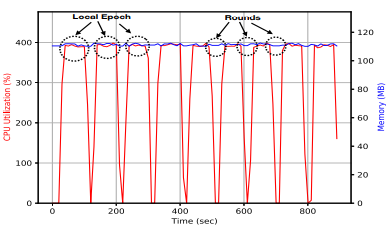
\includegraphics[scale=0.9]{img/fl_CPU_memory.PNG}
\caption{CPU and Memory Consumption}
\label{fig:fl_CPU_memory}
\end{figure}


\textbf{Training time and Temperature}: When comparing the average training time for different numbers of workers, the training time increases significantly as the number of employees increments because the server waits for all clients to report back their freshly trained model (depicted in Figure \ref{fig:fl_time_temperature}).

\begin{figure}[H]
\centering
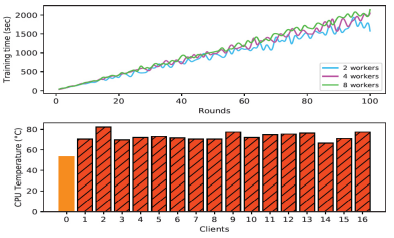
\includegraphics[scale=0.9]{img/fl_time_temperature.PNG}
\caption{Training Time and Device Temperature}
\label{fig:fl_time_temperature}
\end{figure}

